\section{Корреляционный анализ метрик}

Для выявления взаимосвязей между метриками и определения наиболее информативных признаков для прогнозирования целевой переменной $common\_cad$ проведен корреляционный анализ временных рядов.

\subsection{Матрица корреляций Пирсона}

Вычисление коэффициентов корреляции Пирсона между всеми парами метрик позволяет оценить степень линейной взаимосвязи между переменными. Результаты анализа представлены в виде тепловой карты корреляций.

\begin{figure}[H]
	\centering
	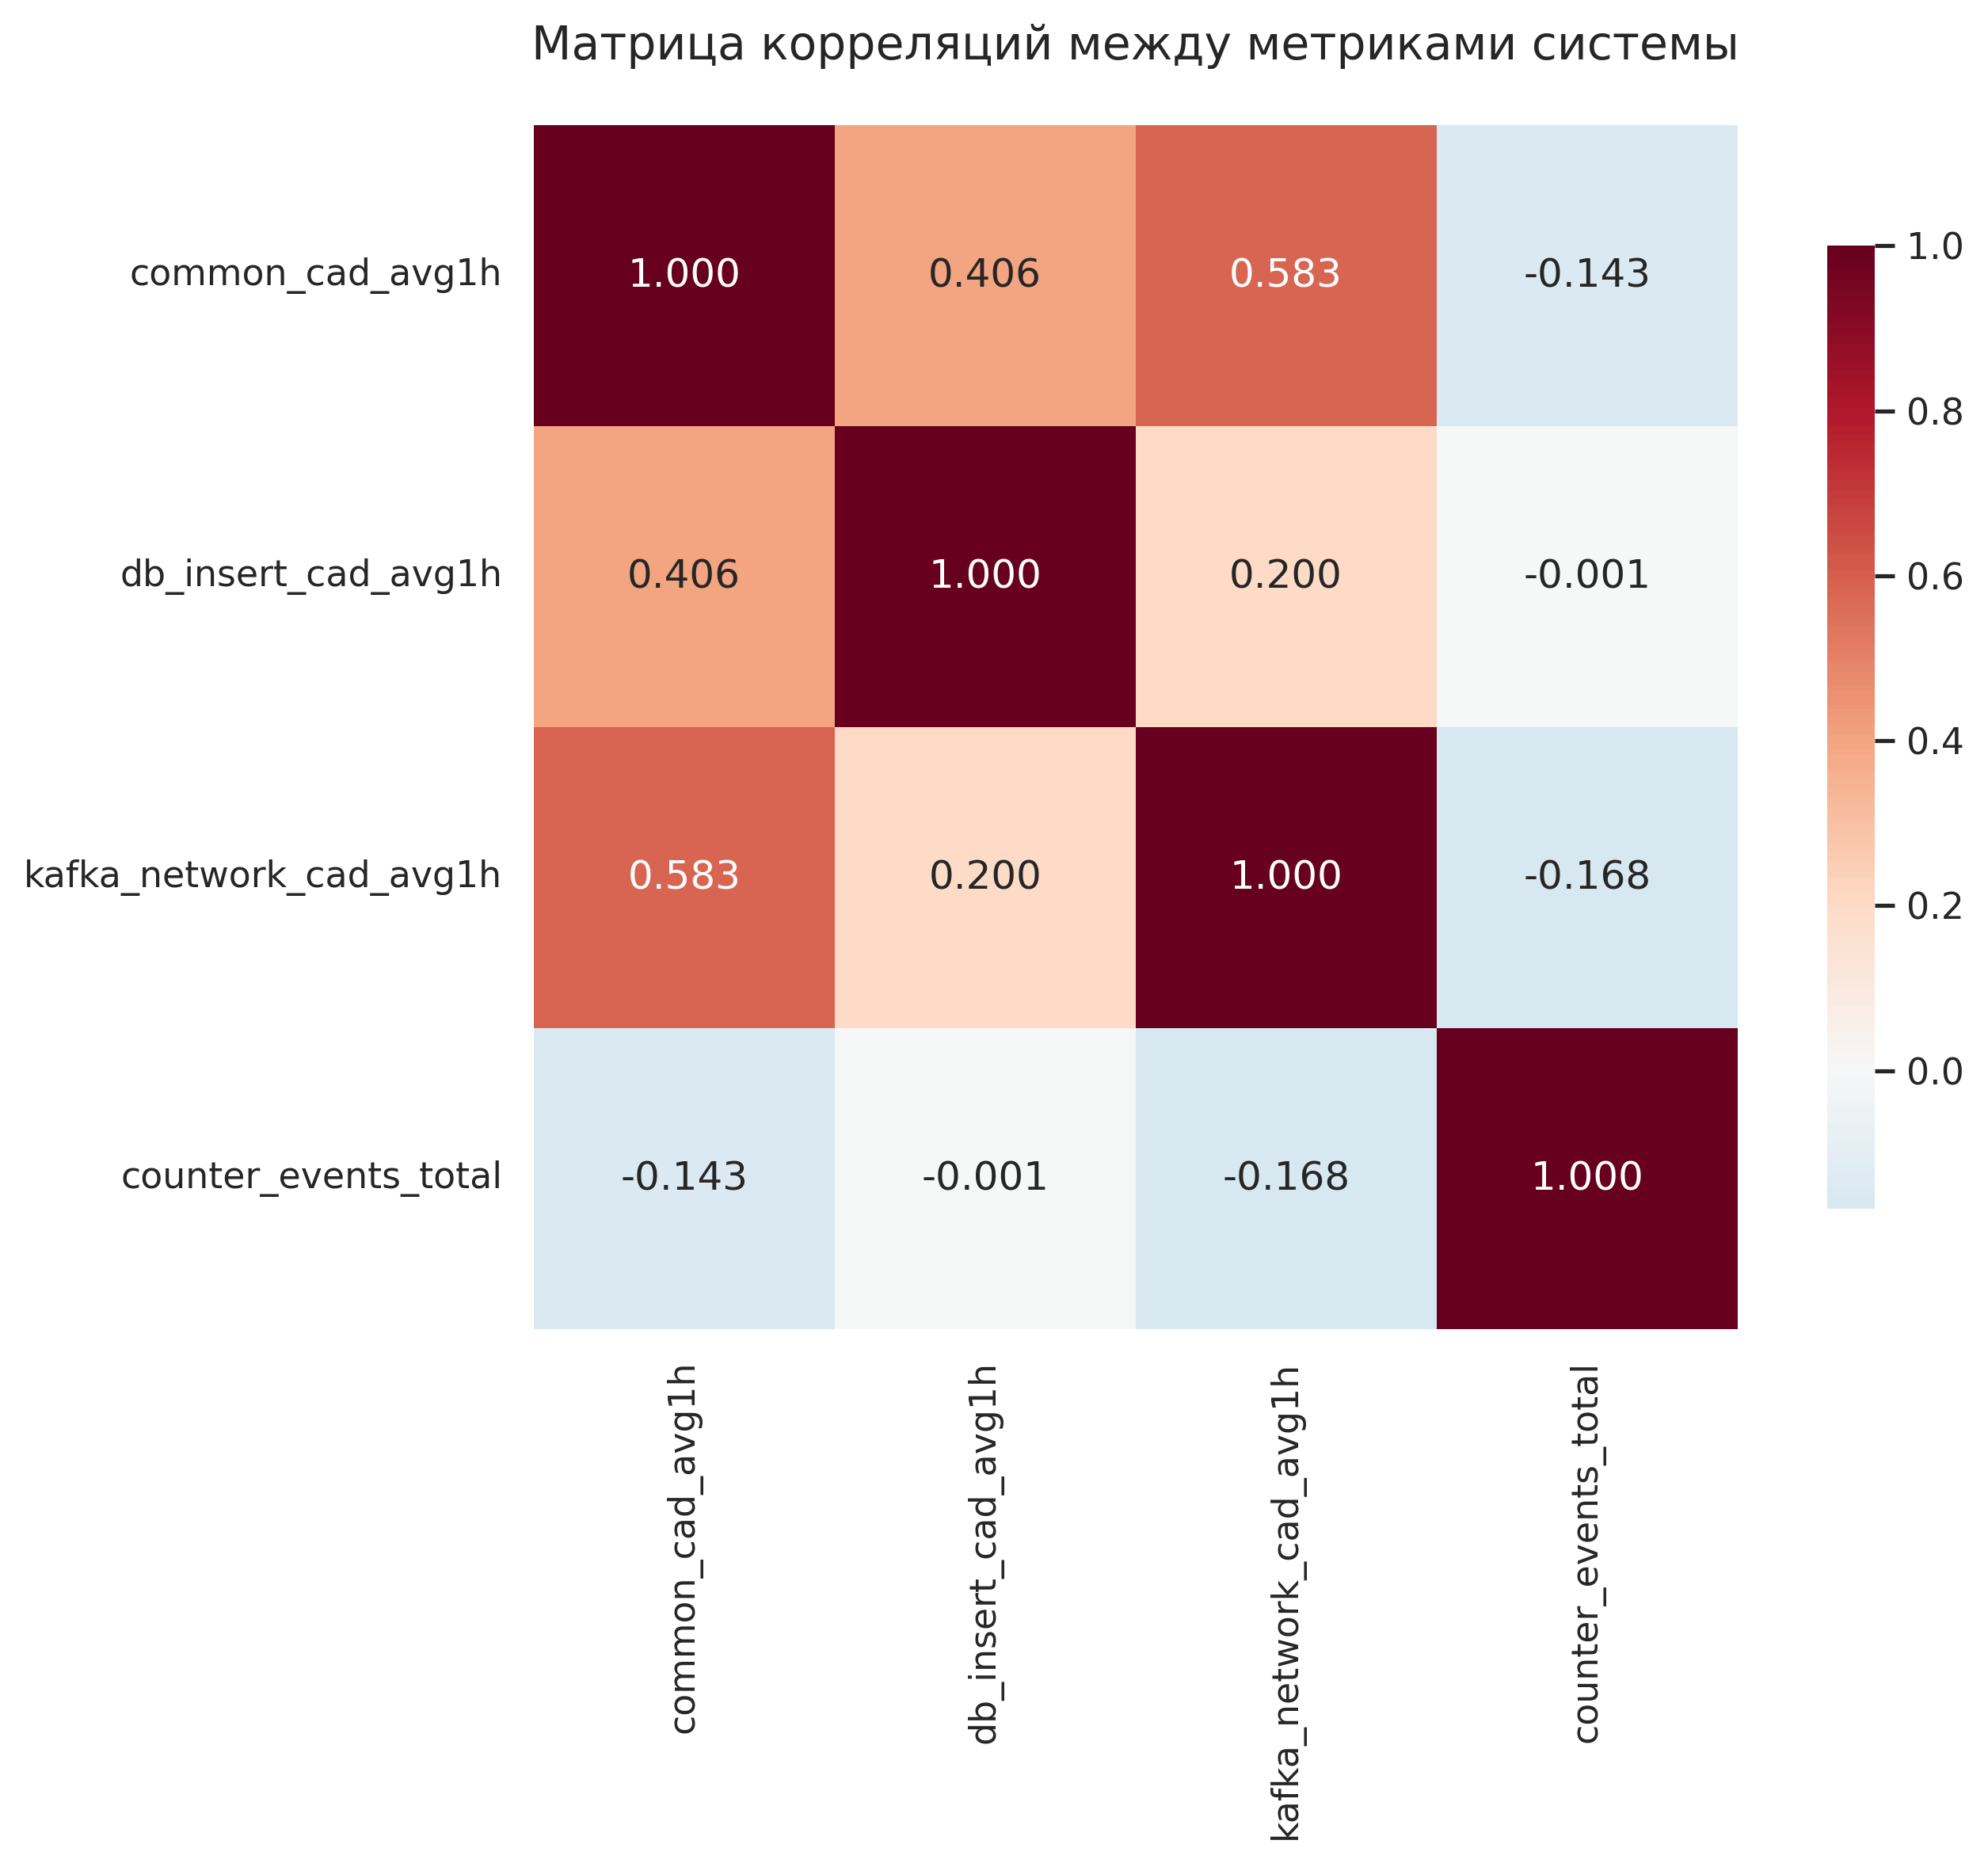
\includegraphics[width=0.7\textwidth]{figures/chapter2/correlation_matrix_heatmap.png}
	\caption*{Рисунок~2.4 --- Матрица корреляций между метриками системы}
	\label{fig:correlation_matrix}
\end{figure}

Анализ матрицы корреляций, представленной на \textit{рисунке 2.4}, показывает наличие значимых взаимосвязей между отдельными метриками, что свидетельствует о взаимозависимости различных компонентов видеоконвейера. Наиболее сильные корреляции наблюдаются между метриками задержек ($common\_cad$, $db\_insert\_cad$, $kafka\_network\_cad$), что логично с точки зрения архитектуры системы.

\subsection{Анализ связей с целевой переменной}

Особое внимание уделено корреляциям с целевой метрикой \\
$common\_cad\_avg1h$, поскольку они определяют потенциальную предсказательную способность признаков. Основные коэффициенты приведены в \textit{таблице 2.2}.

\begin{table}[H]
	\centering
	\caption*{Таблица 2.2 --- Корреляции метрик с целевой переменной $common\_cad\_avg1h$}
	\begin{tabular}{|l|c|}
		\hline
		\textbf{Метрика} & \textbf{Корреляция с $common\_cad\_avg1h$} \\
		\hline
		$kafka\_network\_cad\_avg1h$ & +0.583 \\
		$db\_insert\_cad\_avg1h$ & +0.406 \\
		$counter\_events\_total$ & -0.143 \\
		\hline
	\end{tabular}
	\label{tab:target_correlations}
\end{table}

\subsection{Анализ временной структуры рядов}

Для более глубокого понимания временных зависимостей был проведен анализ автокорреляционной функции (ACF), частной автокорреляционной функции (PACF) и сезонная декомпозиция для ключевых временных рядов.

\subsubsection{Сезонная декомпозиция}

Сезонная декомпозиция позволяет разложить временной ряд на три компоненты: тренд, сезонность и остаток (шум). Это помогает выявить долгосрочные тенденции и периодические колебания в данных. На \textit{рисунке 2.5} представлена декомпозиция для целевой метрики $common\_cad\_avg1h$.

\begin{figure}[H]
	\centering
	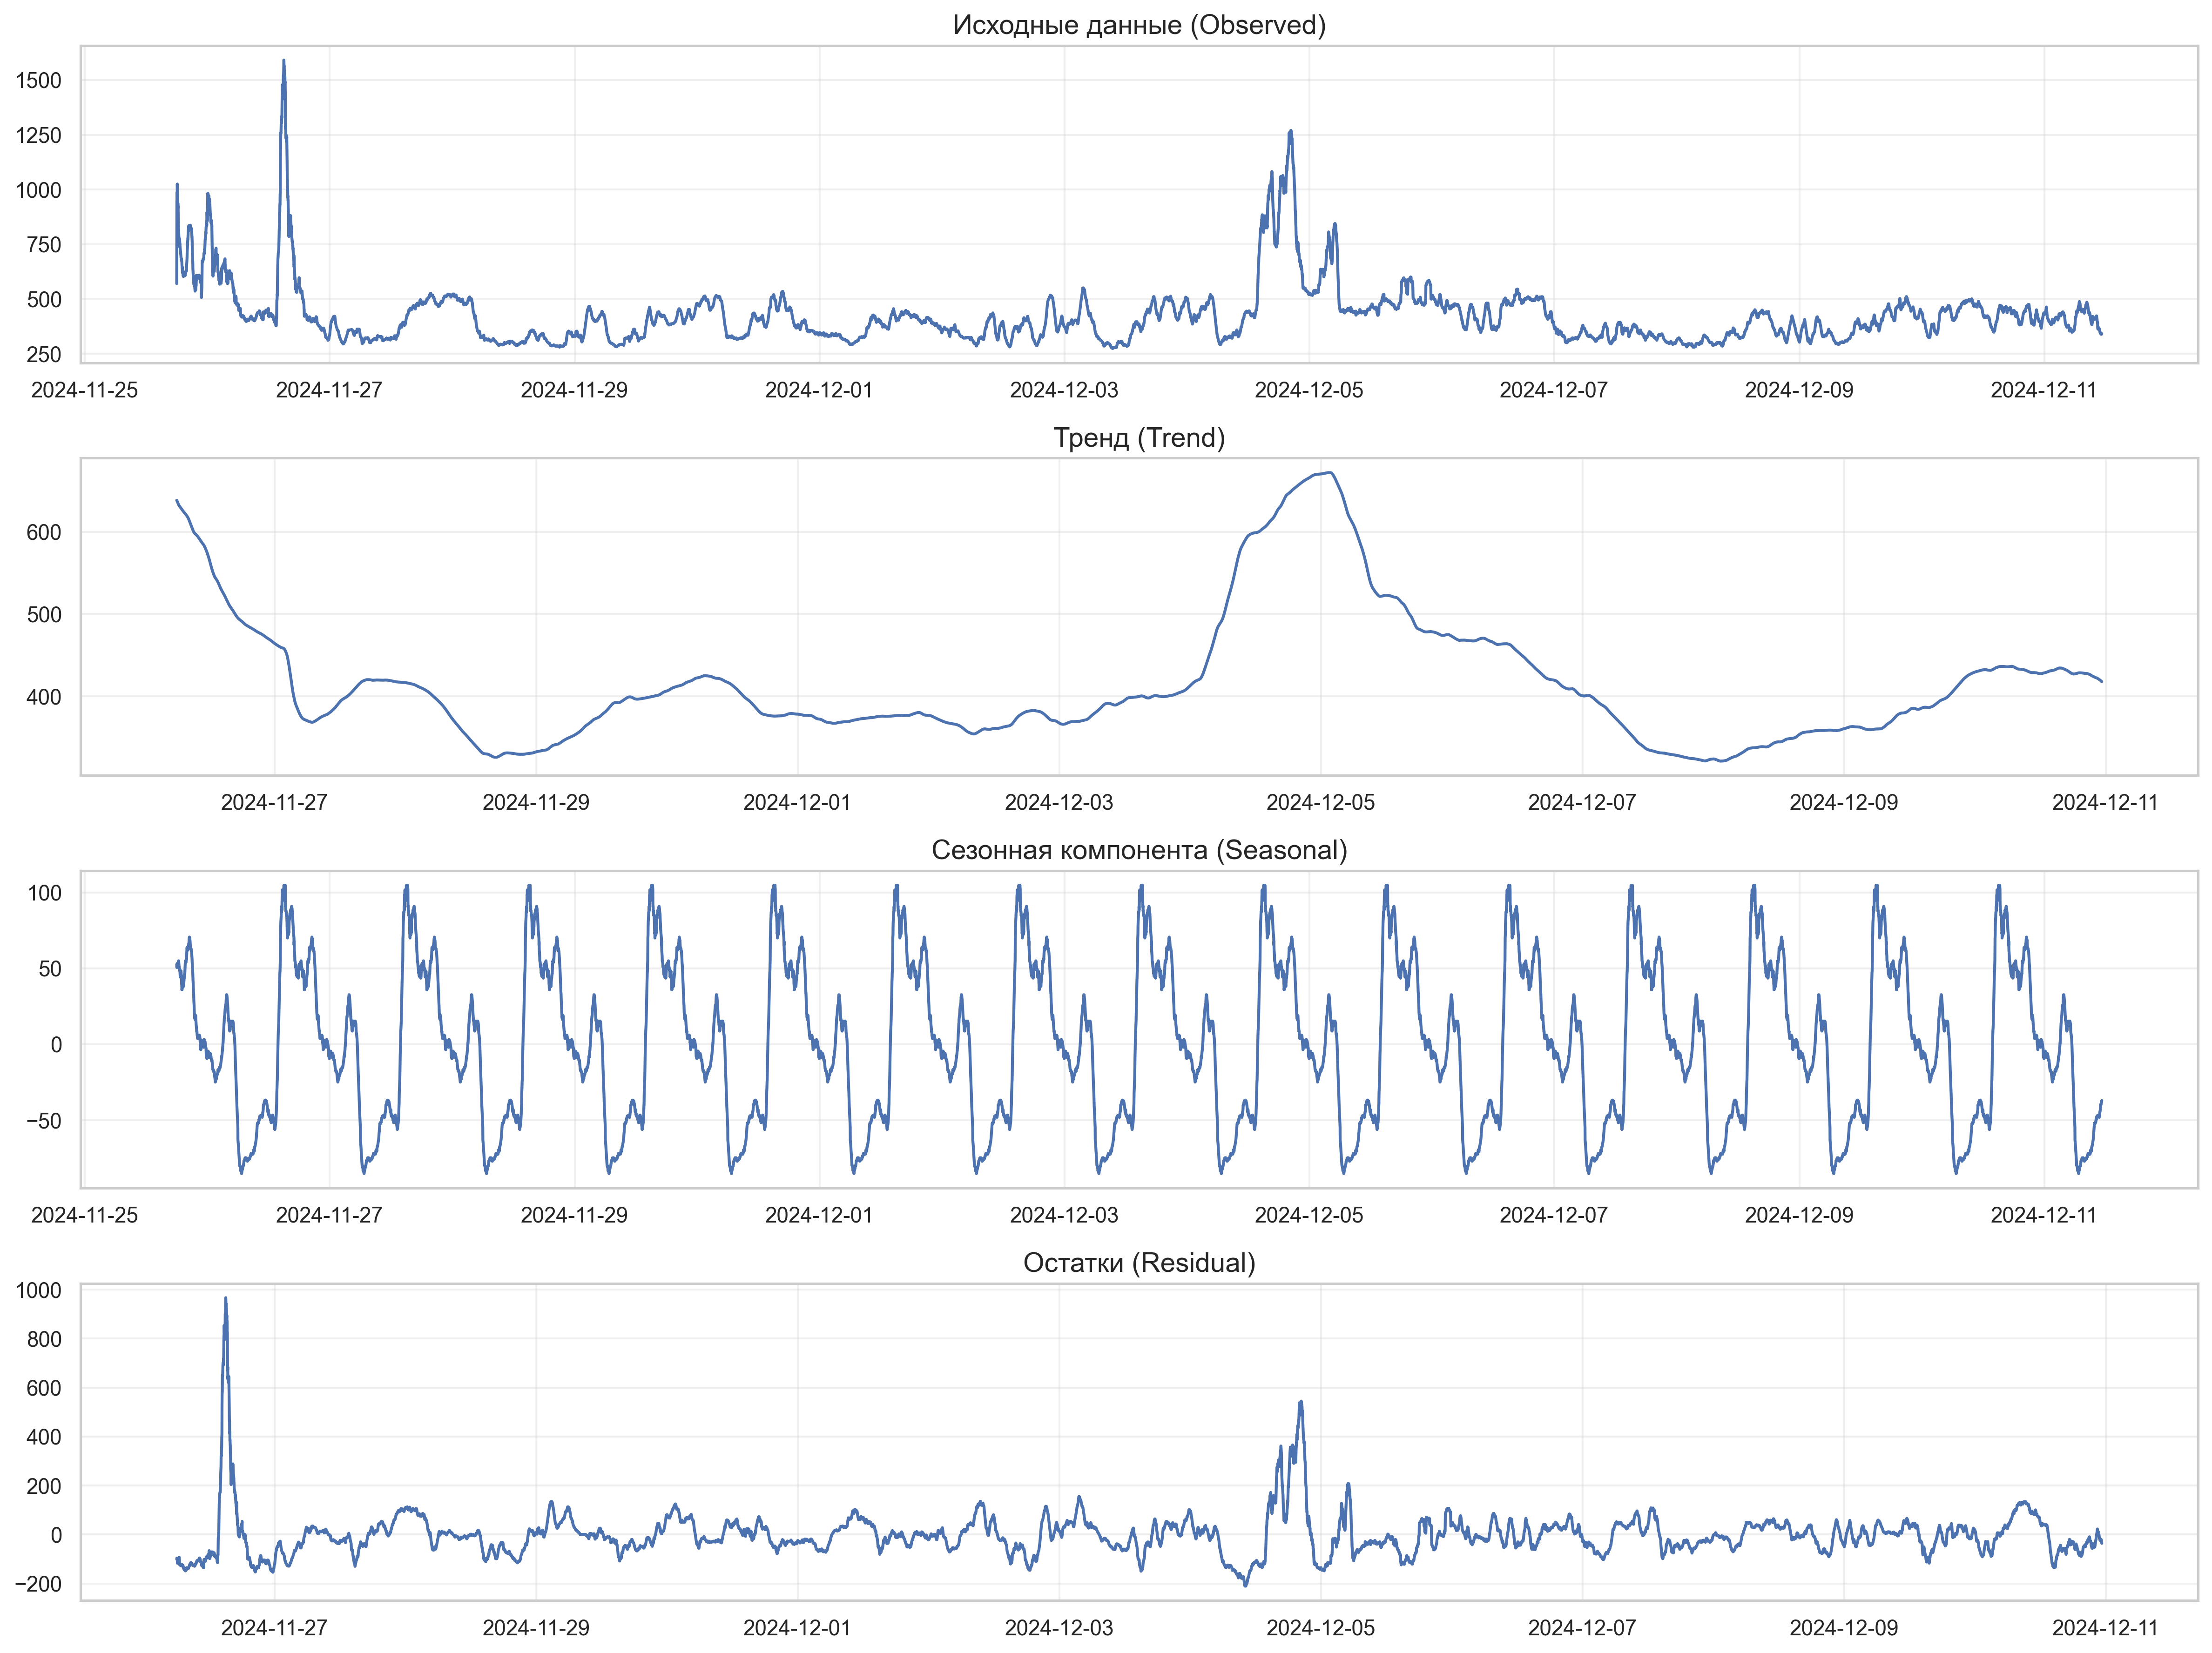
\includegraphics[width=\textwidth]{figures/chapter2/seasonal_decomposition.png}
	\caption*{Рисунок~2.5 --- Сезонная декомпозиция метрики $common\_cad\_avg1h$}
	\label{fig:seasonal_decomposition}
\end{figure}

Анализ показывает наличие выраженного нелинейного тренда с характерным ростом в начале декабря и последующим спадом. Наиболее важной особенностью является доминирующая суточная сезонность с четким повторяющимся паттерном, что характерно для систем с циклической нагрузкой. В остатках наблюдаются аномальные выбросы (например, 26.11 и 04.12), которые модель декомпозиции не смогла объяснить трендом и сезонностью.

\subsubsection{Анализ автокорреляций}

Функции ACF и PACF используются для определения порядка авторегрессионных (AR) и скользящих средних (MA) компонентов в моделях временных рядов, таких как ARIMA. На \textit{рисунке 2.6} показаны графики ACF и PACF.

\begin{figure}[H]
	\centering
	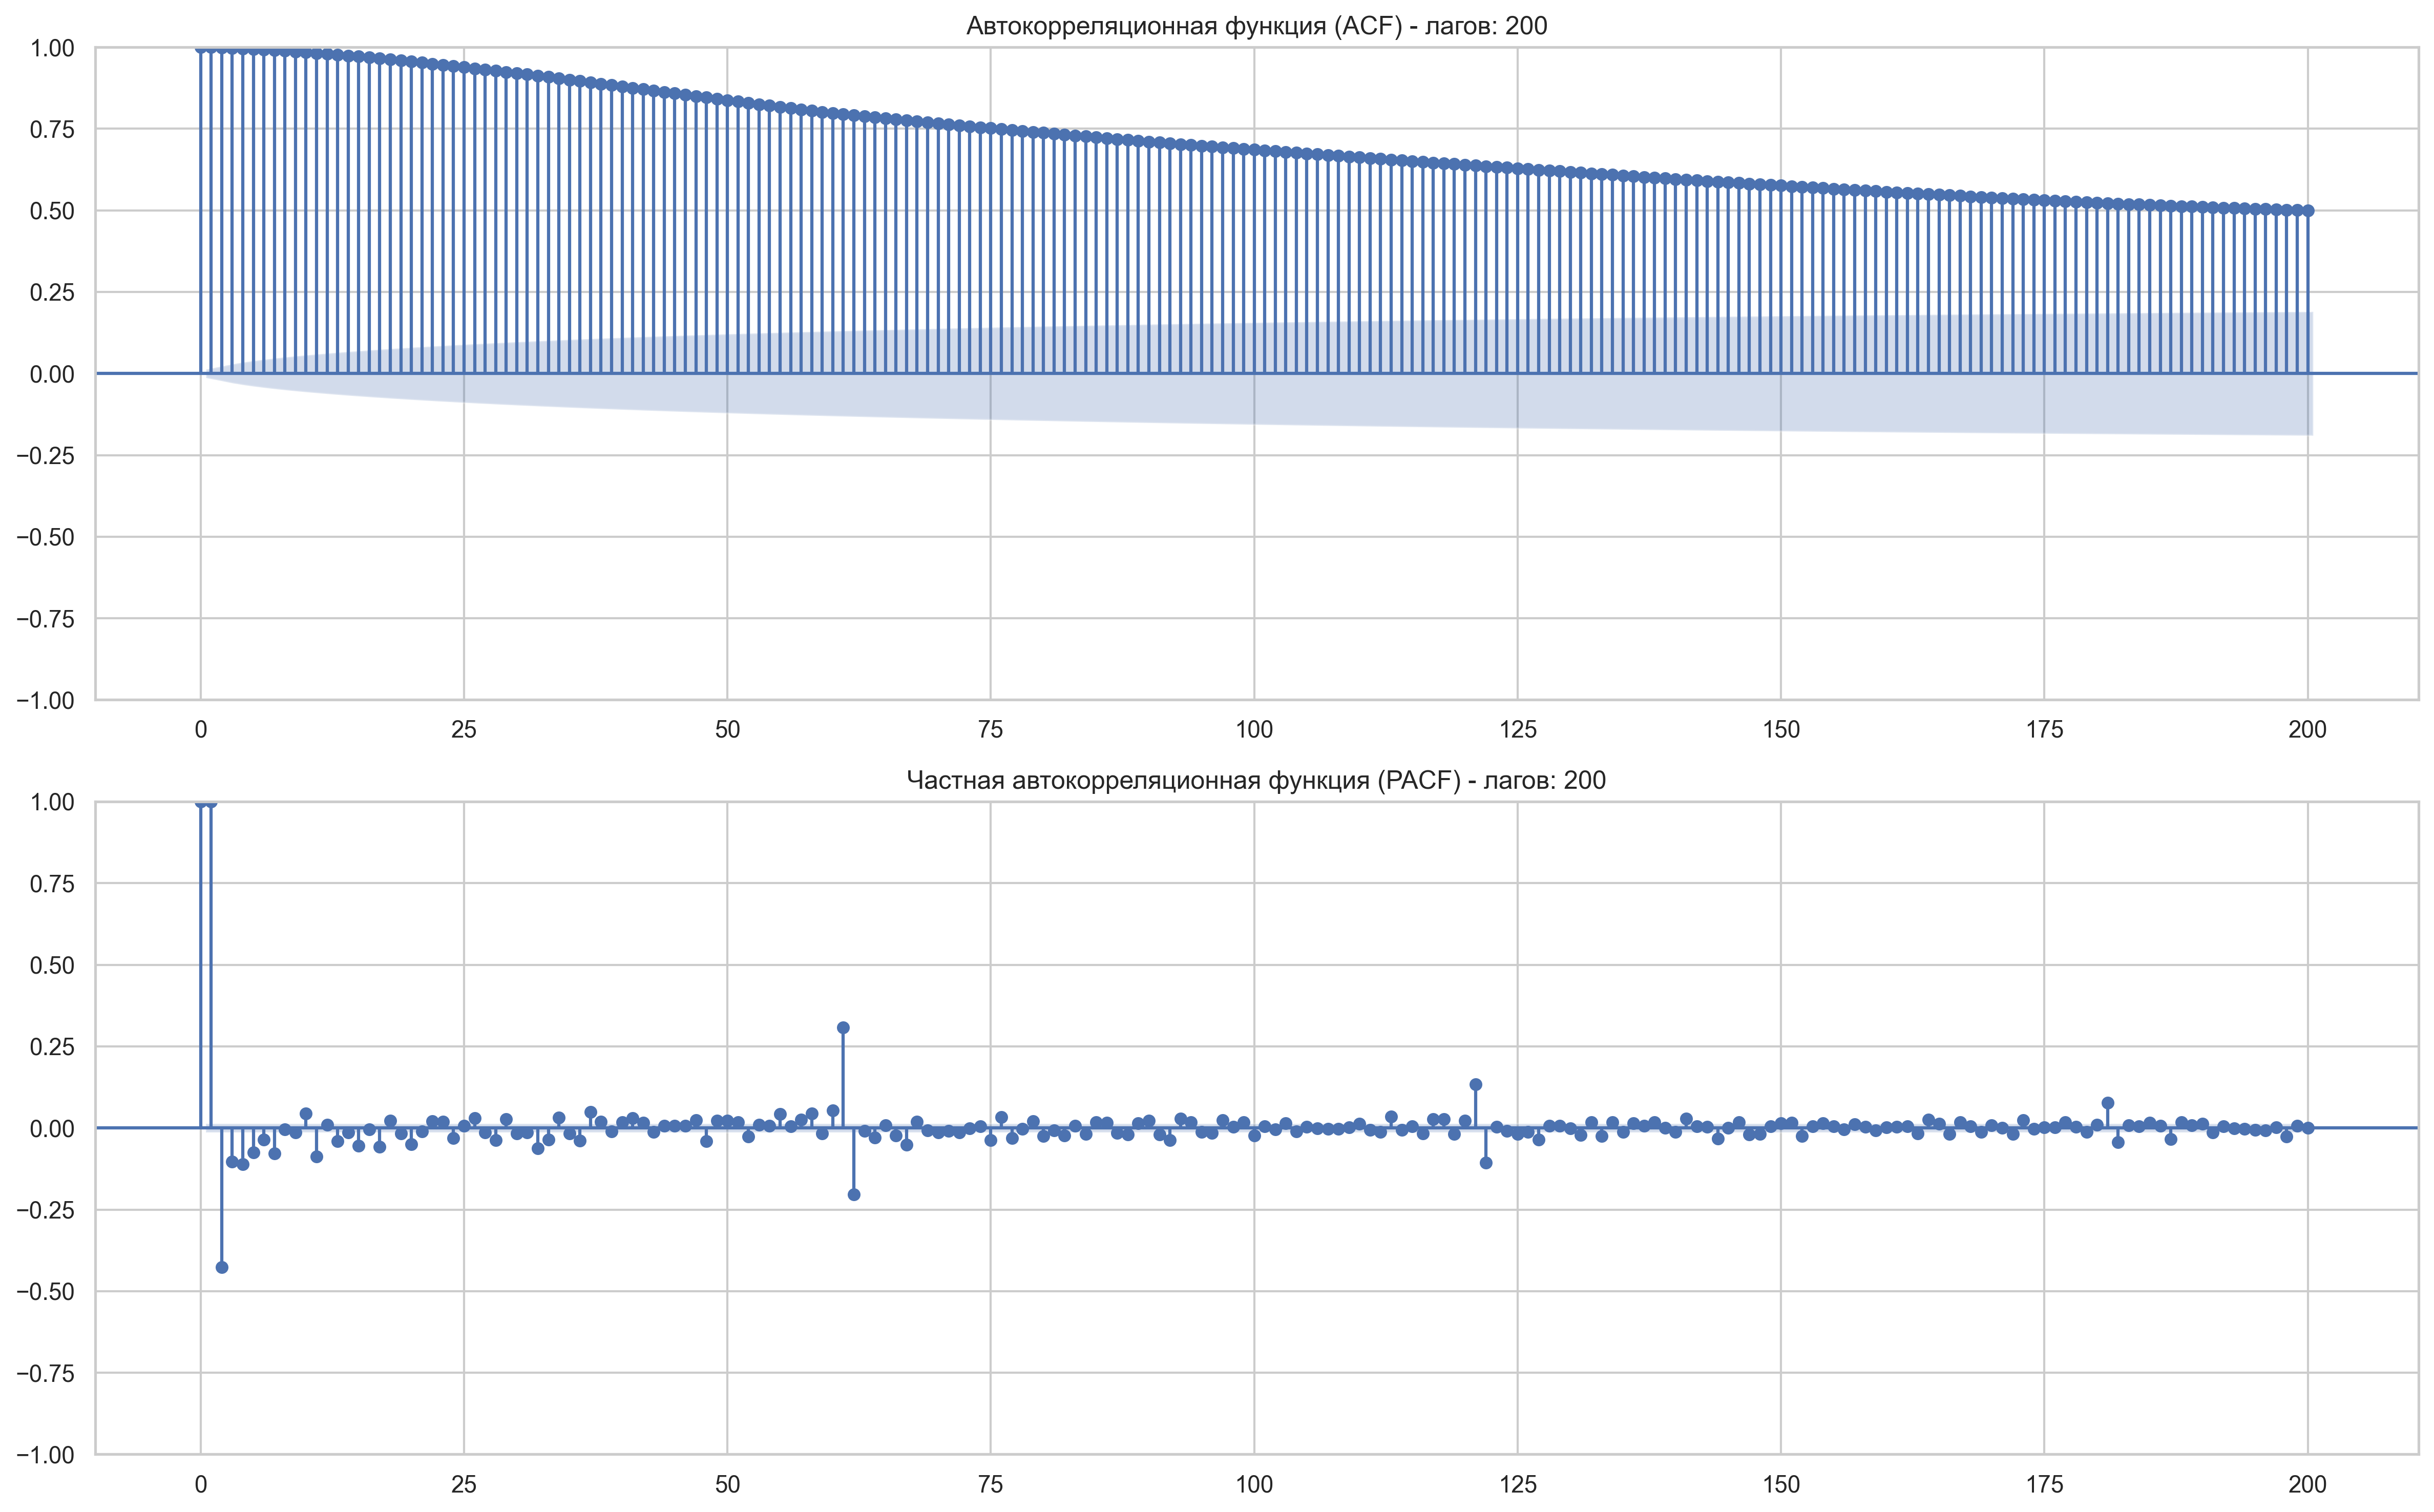
\includegraphics[width=\textwidth]{figures/chapter2/acf_pacf_plots.png}
	\caption*{Рисунок~2.6 --- Графики ACF и PACF для метрики $common\_cad\_avg1h$}
	\label{fig:acf_pacf}
\end{figure}

Анализ автокорреляционных функций выявил ключевые характеристики временного ряда:

\begin{itemize}
	\item \textbf{ACF медленно убывает} на протяжении всех 200 лагов, что является классическим признаком нестационарности ряда и наличия тренда. Волнообразная структура ACF подтверждает сильную сезонность;
	\item \textbf{PACF имеет резкий всплеск на лаге 1} с последующим обрывом, что указывает на авторегрессионный процесс первого порядка (AR(1)). Это означает сильную зависимость текущего значения от предыдущего;
	\item Совместный анализ ACF/PACF предполагает использование модели \\SARIMA с начальными параметрами $p=1$, $d=1$, $q=0$ для несезонной части и дополнительными сезонными параметрами.
\end{itemize}

Однако учитывая сложность выявленных паттернов (нелинейный тренд, аномалии, сильная сезонность), для достижения высокой точности прогнозирования целесообразно рассмотреть как классические статистические методы (SARIMA), так и современные подходы машинного обучения (LSTM, Transformer), способные улавливать нелинейные зависимости.

\subsection{Выводы по итогам анализа данных}

На основе проведенного анализа данных сделаны следующие выводы:

\begin{itemize}
	\item Корреляционный анализ подтвердил наличие статистически значимой связи между системными метриками и целевой переменной. Наиболее сильное влияние оказывает задержка в Kafka ($kafka\_network\_cad\_avg1h$) с корреляцией +0.583, что логично с точки зрения архитектуры системы;
	\item Сезонная декомпозиция выявила доминирующую суточную сезонность и нелинейный тренд с пиком в начале декабря. Обнаружены аномальные выбросы, требующие специальной обработки при моделировании;
	\item Анализ ACF/PACF показал нестационарность ряда (медленно убывающая ACF) и авторегрессионную структуру первого порядка (резкий обрыв PACF после лага 1). Это указывает на возможность применения модели SARIMA(1,1,0) с сезонными компонентами;
	\item Сложность выявленных паттернов (нелинейность, аномалии, сильная сезонность) обосновывает необходимость сравнения классических статистических методов с современными подходами машинного обучения;
	\item Отсутствие сильной мультиколлинеарности между признаками позволяет использовать их все в модели без предварительного отсева.
\end{itemize}

Полученные результаты формируют основу для этапа feature engineering и выбора архитектуры модели прогнозирования, которые будут рассмотрены в следующей главе.

